%Arquitectura de Control
\chapter{Plataformas Experimentales}\label{sec:capitulo4}
\thispagestyle{empty}
En este capítulo se explican las plataformas experimentales utilizadas para el desarrollo y validación de los algoritmos propuestos en el presente trabajo, las cuales fueron: Matlab y Dynacar. Donde la herramienta de Matlab fue empleada para la realización de los códigos,  y conjunto a su entorno de simulación, Simulink se implementaron los bloques que conforman la arquitectura de control de los vehículos, más específcamente los relacionados a las comunicaciones V2V y maniobras cooperativas, para luego ser utilizdos y validados en el simulador Dynacar. Es por esto que a continuación se detallará de mejor forma cada una de estas plataformas.\\
\section{Software Matlab}
MATLAB\footnote{https://la.mathworks.com/products/matlab.html/} es una herramienta de software matemático que ofrece un entorno de desarrollo integrado, IDE (del inglés, \textit{Integrated Development Environment}), que cuenta con diversas prestaciones como la manipulación de matrices, implementación de algoritmos, creación de interfaces gráficas de usuario, GUI (del inglés, \textit{Graphical User Interface}) y la comunicación con programas en otros lenguajes y otros dispositivos de hardware. Debido a su capacidad de desempeño asíncrono permite manejar fuentes heterógeneas de datos, como sensores, sistemas de comunicación, etc, sin nunguna restricción. Teniendo en cuenta estas cualidades, el MATLAB permite a ingenieros e investigadores utilizar las ventajas de un software eficiente y fácil de usar en aplicaciones que necesitan desarrollos rubustos y de procesamiento rápido.\\
\par En este trabajo se empleó la versión 2016a \footnote{https://la.mathworks.com/company/newsroom/mathworks-announces-release-2016a-of-the-matlab-and-simulink-product-families.html/} de MATLAB, disponible desde el 21 de marzo de 2016, la cual cuenta con numerosas mejoras con respecto a sus antecesoras, como por ejemplo: la inclusión y correción de distintos toolbox relacionados al área de control, así como también el perfeccionamiento en las técnicas de depuración de código. Este IDE posee cuatro ventanas, como se muestra en la figura \ref{fig:ide}.\\

\begin{figure}[!h]
	\centering
		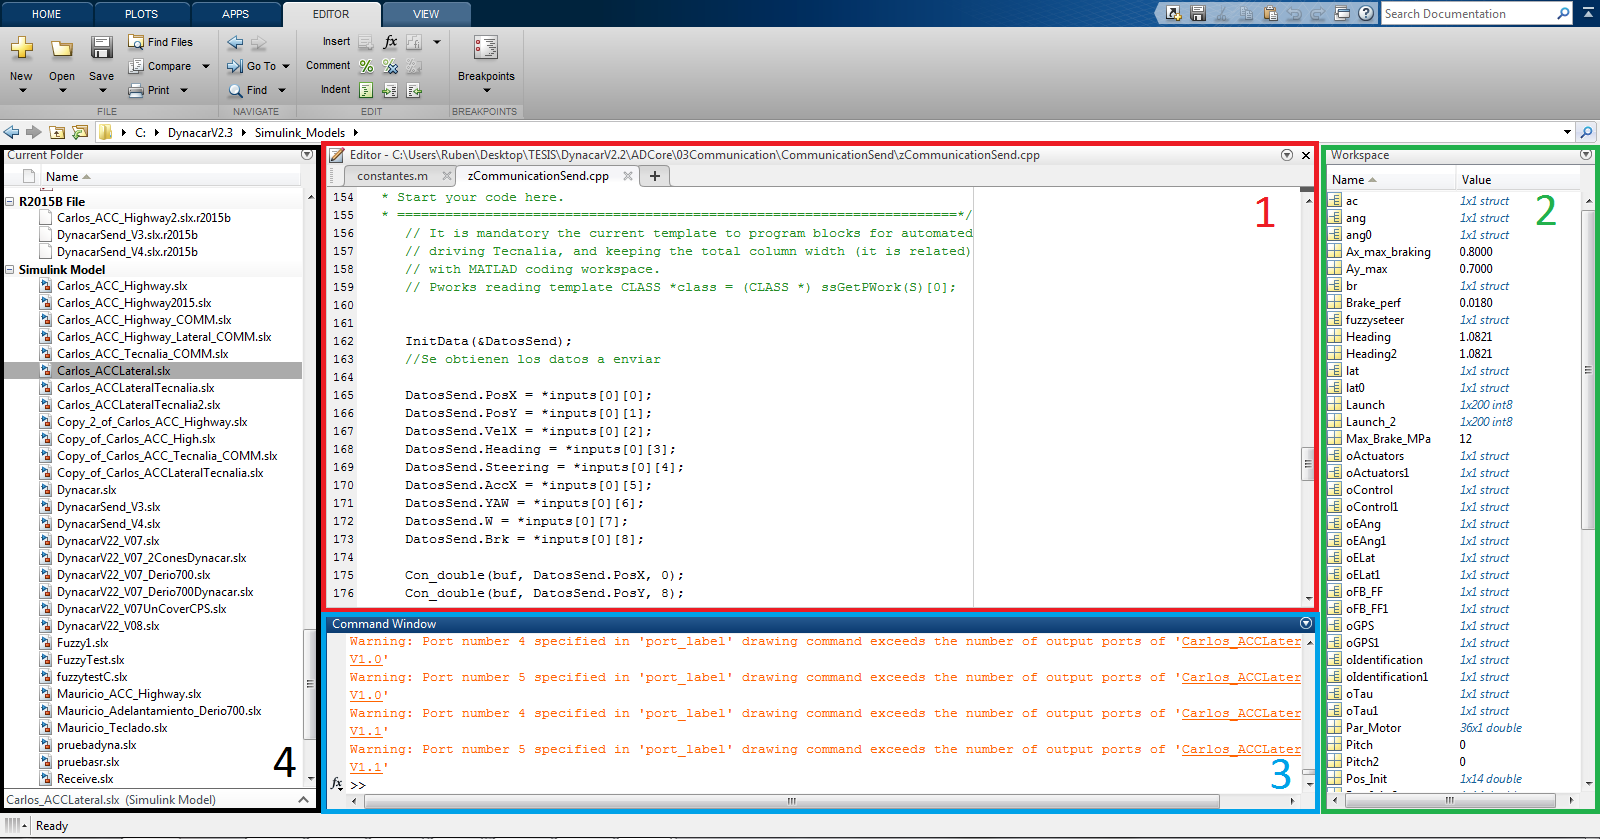
\includegraphics[scale=0.3]{Imagenes/ide}
		\caption{IDE de MATLAB}
		\label{fig:ide}
\end{figure}	 
\par Donde:\\
\begin{enumerate}
    \item Editor de texto: es donde se crean programas y funciones, para luego ser compiladas y ejecutadas. 
    \item Espacio de trabajo: es donde se muestran todas las variables y estructuras creadas, las cuales pueden ser manipuladas tanto con la ventana de comandos como con el editor de texto.
    \item Ventana de comandos: es donde se pueden escribir y ejecutar líneas de código directamente.
    \item Carpeta actual: es donde se muestra la carpeta actual, con sus respectivos archivos.
\end{enumerate}
\par Este software emlea su propio lenguaje de programación, el lenguaje M, pero a través de compiladores como Mingw32, se pueden utilizar otros lenguajes como C o C++. Lo que da paso a la utilización de otras características como lo son el uso de las S-Function, funciones de suma importancia en el esquema de Dynacar, ya que permiten crear bloques de simulink, empleando algoritmos realizados en lenguajes como C, C++ y Fortran.\\
\par Para la realziación de los bloques del sistema de comunicación se empleron las S-Function, conjunto a la libreria de Sockets para Windows de lenguaje C. Libreria que permite el uso de los sockets, que son enlaces punto a punto, que permiten comunicar una computadora con otra. Dichos enlaces pueden ser de dos tipos: Stream Sockets y Datagram Sockets, siendo basados cada uno en los protocolos de trasnporte TCP y UDP respectivamente. Ya habiendo explicado el software MALTAB, ahora se procederá a descrbir la herramienta, Simulink
\subsection{Simulink}
Simulink es una herramienta de MATLAB hecha para modelar, simular y analizar sistemas dinámicos. Soporta tanto sistemas lineales como no lineales, modelando tiempo continuo, tiempo discreto o en forma mixta. Estas características resultan favorables para la implementación de la arquitectura de control por medio de bloques. En la figura \ref{fig:sim} se puede ver la interfaz gráfica de Simulink, interfaz que se basa en una amplia biblioteca de componentes con entradas y salidas que se pueden interconectar entre sí. Este editor gráfico permite crear y gestionar bloques jerárquicos, es decir se puede tener diagrama principal y dentro del mismo tener diagramas secundarios, cualidad de gran utilidad para la independización de los módulos de comunicación.\\ 

\begin{figure}[!h]
	\centering
		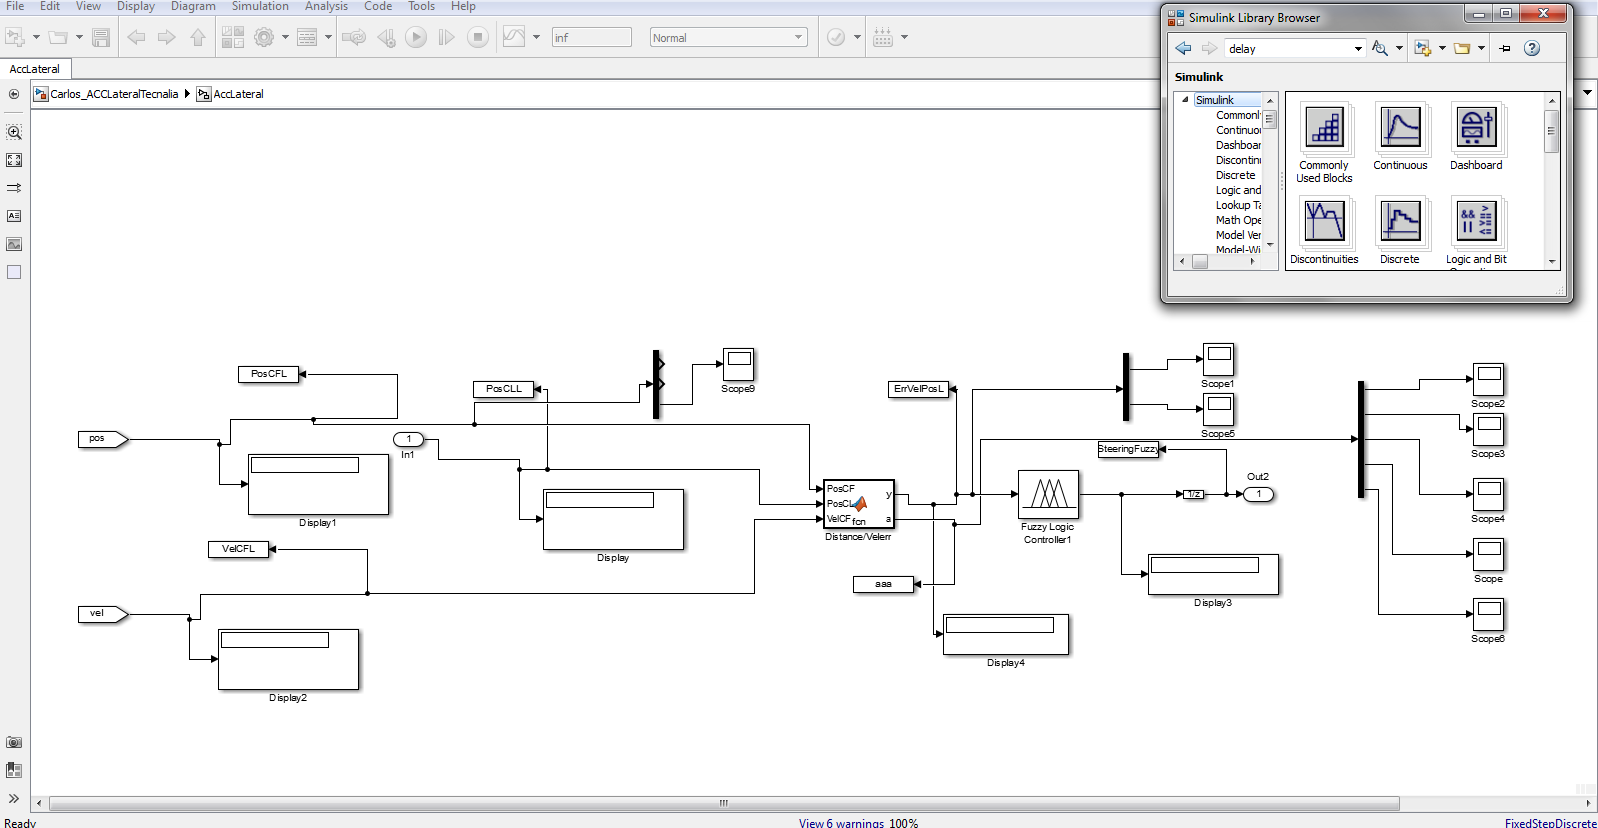
\includegraphics[scale=0.3]{Imagenes/sim}
		\caption{IDE de Simulink}
		\label{fig:sim}
\end{figure}	
\section{Simulador Dynacar}
Dynacar\footnote{http://www.dynacar.es/en/home.php es software}, desarrollado por Tecnalia en la pataforma de LabVIEW, es un software que permite a los ingenieros diseñar y probar modelos completos de vehículos en un ambiente completo y personalizable. Dynacar está compuesto de tres módulos:
\begin{itemize}
	\item Código de la dinámica de vehículos en LabVIEW: son los agoritmos necesarios para el software de prueba, los mismos son ejecutables en tiempo real, y poseen ya, una biblioteca de carros y escenarios de prueba básicos.
	\item Interfaz gráfica de usuario: es la interfaz que permite realizar la parametrización de los vehículos y escenarios (Figura \ref{fig:ste}).
	\item Entorno visual 3D: es el módulo que permite la visualización de las pruebas y del simulador de manejo real del vehículo en el entorno virtual.
\end{itemize}

\begin{figure}[!h]
	\centering
		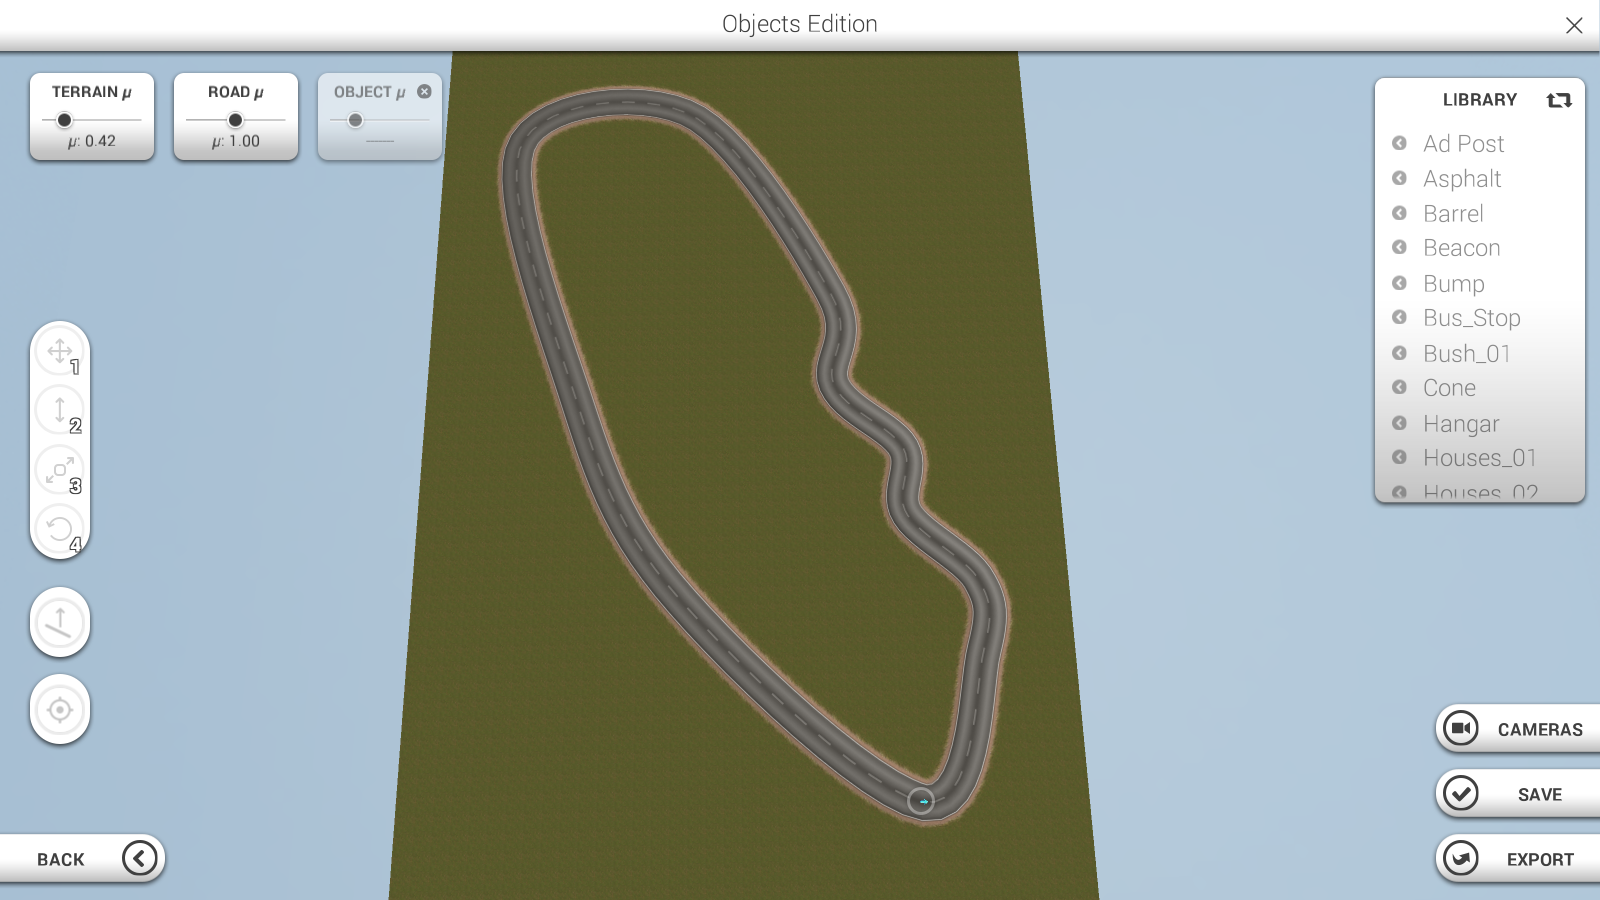
\includegraphics[scale=0.3]{Imagenes/ste}
		\caption{Interfaz gráfica de usuario para la creación de escenarios}
		\label{fig:ste}
\end{figure}	


\par Para poder modelar los vehículos en el simulador, es necesario aportar los siguientes datos:

\begin{itemize}
	\item Masa del vehículo e inercia.
	\item Parámetros de suspensión.
	\item Propiedades de la derección del vehículo.
	\item Características de la aerodinámicas del vehículo.
	\item Propiedades de los neumáticos.
	\item Motor, caja de cambios y propiedades de la transmisión.
	\item Detalles de los actuadores.
\end{itemize}
\par Este simulador se hizo con el objetivo de poder detectar fallos en la ejecución de las maniobras de forma sencilla, y de esta manera poder conocer cuáles son los aspectos que se necesitan ser revisados. Para conseguir este objetivo la plataforma ofrece el entorno visual, el cual se comunica mediante socket de UDP con otras aplicaciones, las cuales envían una trama de datos, con las características del vehículo. En dicho entorno se pueden observar en tiempo real la velocidad lineal en Km/h y la velocidad angular en RPM las ruedas. Además de de estos datos también muestra las acciones sobe los actuadores medidos en porcentajes,junto con la dirección de los vehículos, como se puede apreciar en la Figura \ref{fig:simu}.\\\\\\\\   

\begin{figure}[!h]
	\centering
		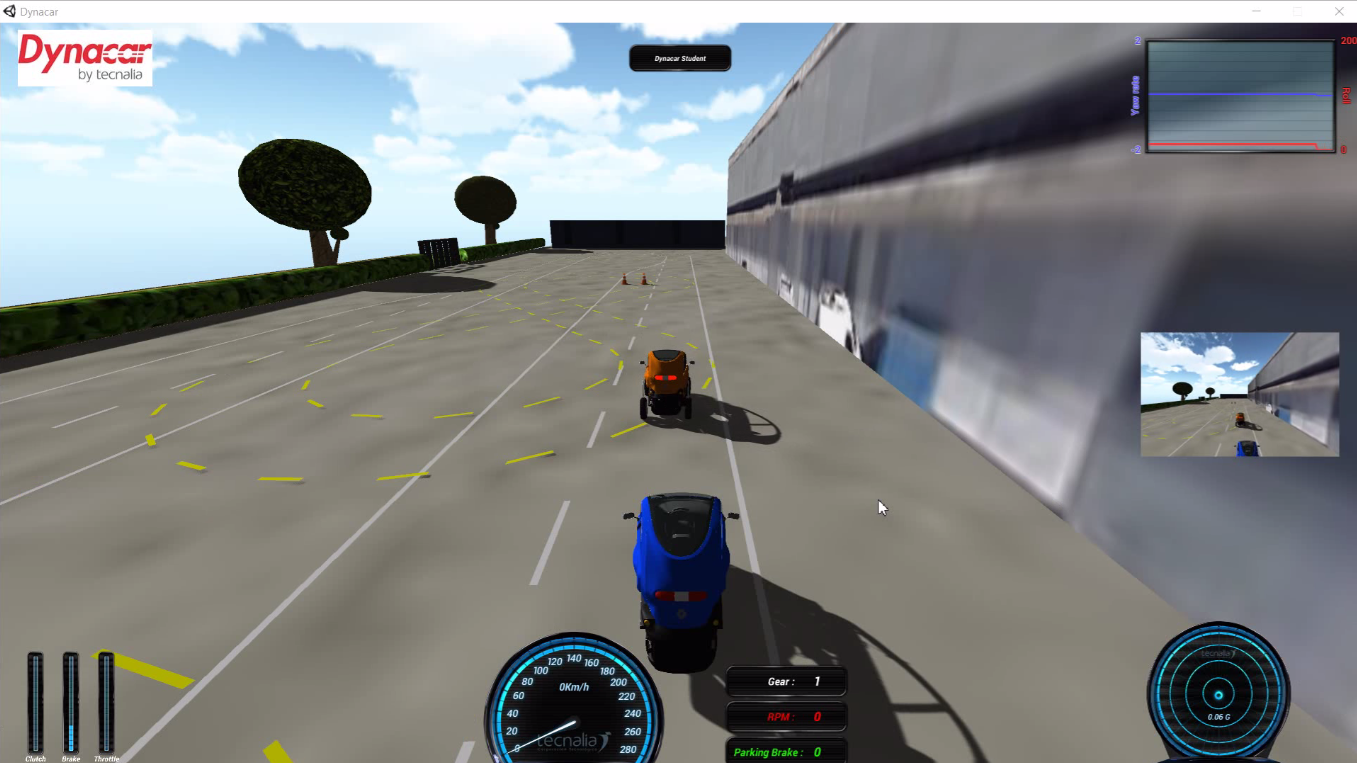
\includegraphics[scale=0.45]{Imagenes/simu}
		\caption{Simulador Dynacar}
		\label{fig:simu}
\end{figure}	

\subsection{Plataformas de Prueba}

A continuación, se presenta una breve descripición de la automatización e instrumentación del Twizy, que corresponde a la plataforma real, así como una explicación de la plataforma virtual, a través de modelos matemáticos.

\subsubsection{Plataforma Real}

Como fue comentado en la sección 2.2.1 para las pruebas reales se emplea el Renault Twizy 80, un vehículo eléctrico, capaz de alcanzar una velocidad máxima de 80 Km/h, el cual ha sido instrumentado de tal forma que el control del volante y de los pedales es realizado a través de una red de bus CAN. Una descripción más detallada de las características físicas del vehículo se puede encontrar en la tabla \ref{tab:cart} \cite{twizyman}\\

\begin{table}[H]
  \centering
\resizebox{\textwidth}{!}{
    \begin{tabular}{|p{16.93em}|c|}
    \toprule
    \multicolumn{1}{|c|}{Características} & Valores \\
    \midrule
    Masa (Kg) & 611.500 \\
    \midrule
    Centro de gravedad X, Y, Z (m) & -0.928, 0, 0.488 \\
    \midrule
    Ancho entre ruedas (m) & 1.686 \\
    \midrule
    Distancia entre el centro de las ruedas delanteras con las traseras & 1.094 \\
    \midrule
    Inercia Ix, Iy, Iz (Kg-m2) & 243.175, 430.166, 430.166 \\
    \midrule
    Radio de las ruedas delanteras (m) & 0,265 \\
    \midrule
    Radio de las ruedas traseras (m) & 0,281 \\
    \midrule
    Torque máximo (N-m) & 57 \\
    \midrule
    Caballos de fuerza (hp) & 11 \\
    \bottomrule
    \end{tabular}}%
  \caption{Características físicas del Twizy 80}
  \label{tab:cart}%
\end{table}%



\par Esta plataforma se puede dividir en tres sistemas manejados por diferentes dispositivos electrónicos y actuadores (Tabla \ref{tab:sen}), los cuales son controlados por un PLC \cite{marcanolow}:

\begin{itemize}
\item Volante: es manejado por un motor de paso, el cual es controlado por señales moduladas por ancho de banda, PWM (del inglés, \textit{Pulse-Width Modulation}). 
\item Acelerador: es controlado por la unidad de control del motor, ECU (del inglés, \textit{Engine Control Unit}), la cual recibe una señal de voltaje analógica entre 0 y 10 VDC. 
\item Freno: es manejado a través de un actuador mecánico lineal.
\end{itemize} 

% Table generated by Excel2LaTeX from sheet 'Hoja1'
\begin{table}[H]
  \centering
\resizebox{\textwidth}{!}{
    \begin{tabular}{|c|c|}
    \toprule
    Data de la Inercia y Posición & \textit{GNSS-aided IMS + Base Station} \\
    \midrule
    OBU   & Fanless - i7-6700TE - 32 GB RAM \\
    \midrule
    \multirow{2}[4]{*}{Sistema de Frenado} & Actuador Lineal - 750 N \\
\cmidrule{2-2}          & Driver de 20 A del Motor DC \\
    \midrule
    \multicolumn{1}{|c|}{\multirow{3}[6]{*}{Sistema del Volante}} & Motor paso a paso híbrido de alto torque \\
\cmidrule{2-2}          & Encóder magnético con CANopen \\
\cmidrule{2-2}          & Driver de 20-80 V del motor paso a paso \\
    \bottomrule
    \end{tabular}}%
  \caption{Sensores y dispositivos electrónicos}
  \label{tab:sen}%
\end{table}%

\subsubsection{Plataforma Virtual}

Dynacar, además del ya descrito Visor 3D, incorpora un modelo multi-cuerpo \cite{cuadrado2013multibody} con el cual se pueden representar los vehículos virtualmente. Dicho modelo hace uso de de coordenadas relativas, así como también ecuaciones semi-recursivas del movimiento, basado en la transformación de la velocidad. Las suspensiones son consideradas como macro-articulaciones, cuyo comportamiento es descrito usando las estructuras de tablas de consulta.\\ 

\par Como se puede apreciar en la figura \ref{fig:mult}, las coordenadas cartesianas del chasis se encuentran en el medio del ancho de las ruedas delanteras (C), los ángulos de navegación  que proveen la orientación de las reudas con respecto al chasis se encuentran en los nudillos (K), y por último, las expresiones cinemáticas para las macro-articulaciones consideran, tanto la posición, como la velocidad y aceleración de las ruedas (W).\\

\begin{figure}[!h]
	\centering
		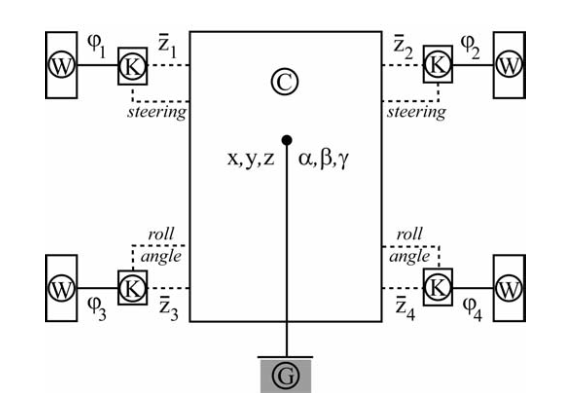
\includegraphics[scale=0.7]{Imagenes/mult}
		\caption{Modelo multi-cuerpo de Dynacar \cite{cuadrado2013multibody}}
		\label{fig:mult}
\end{figure}	      


\subsection {Arquitectura de control}
La arquitectura de control utilizada está compuesta por seis bloques representativos de cada módulo de interés dentro de la conducción automatizada (Figura \ref{fig:fram}), estos son: Adquisición, Percepción, Control, Comunicación, Desición y Actuación. Esta arquitectura ha sido utilizada en distintas aplicaciones de conducción autónoma, como por ejemplo, en \cite{lattarulo2017complete} y \cite{sriranjanlateral}. Siendo en el primero, usada para probar distintas metodologías, con el fin de validar distintos algoritmos de control y de planificación de ruta, mientras que para el segundo es implementada en autentificación de distintos algortimos de control lateral. Cada módulo es detallado a continuación:

\begin{figure}[!h]
	\centering
		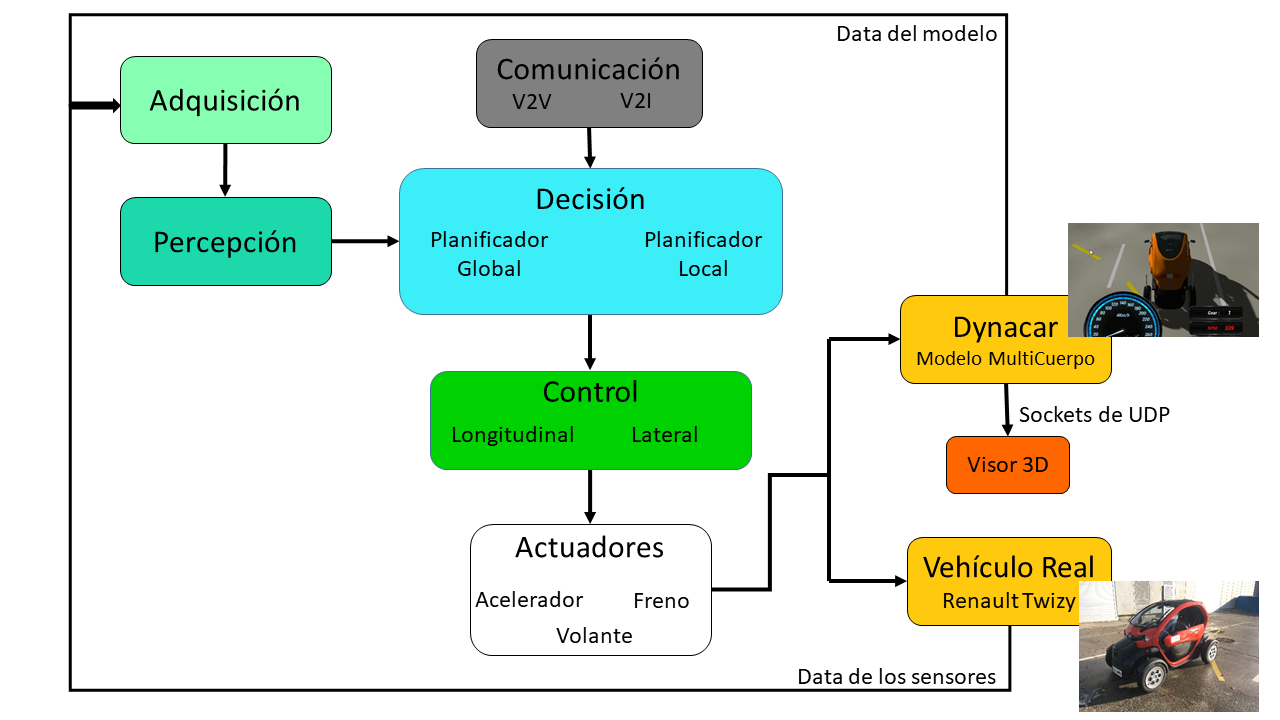
\includegraphics[scale=0.4]{Imagenes/fram}
		\caption{Arquitectura de control}
		\label{fig:fram}
\end{figure}	

\begin{itemize}
	\item Adquisición: es el bloque responsable de generar las señales de posición, velocidad, y demás información referente a la dinámica del vehículo. Estos datos son obtenidos a través del modelo multi-cuerpo que representa el vehículo simulado. En el caso de los vehículos reales este bloque reune y realiza las tareas de pre-procesamiento de la información proveniente de distintos dispositivos, como lo son: los distintos sensores, la unidad de medición inercial, IMU (del inglés, \textit{Intertial Measurement Unit}), el GPS diferencial, entre otros.  
	\item Comunicación: es el módulo encargado de simular las comunicaciones V2X, característica importante para la prueba de maniobras más complejas. Esta plataforma es de gran utilidad para simular las interacciones de los vehículos con las infraestructuras. En este bloque se enfocó el presente trabajo, incorporando a la arquitectura un bloque para enviar la trama de datos, la cual consta de la posición,velocidad, ángulo de dirección, tiempo y el valor de los actuadores, así como un bloque de recepción de datos. Además de los ya mencionados se agregó un bloque con el cual se puede observar en el visor 3D, el vehículo con el cual se esta realizando la comunicación.    
	\item Percepción: es el módulo responsable de recolectar la data de los módulo de adquisición, armando así un paquete con la información y los parámetros de configuración del vehículo, el cual es trasladado a los bloques de decisión y control. Dentro de la información a envíar, se pueden destacar: la estimación del ego-vehicle, la detección y/o clasificación de objetos, detección de carril, y la detección de señales de tráfico. 
	\item Decisión: es el bloque encargado de generar la ruta por donde se va a transitar, para lo cual el módulo se divide en dos sub módulos, el planificador global y el planificador local.
	\begin{itemize}
	\item Planificador global: es el encargado de generar la ruta que va a seguir el vehículo (Figura \ref{fig:gp}). Para crear la ruta el bloque considera la información tanto del punto de partida como del punto de llegada, así como también la información proveniente del bloque de HMI, que puede cambiar el camino de forma dinámica. Esta ruta tiene que ser lo suficientemente precisa para que el planificador local pueda generar trayectoria suave, que, además tome en cuenta escenarios urbanos, como intersecciones, rotondas, etc.

\begin{figure}[!h]
	\centering
		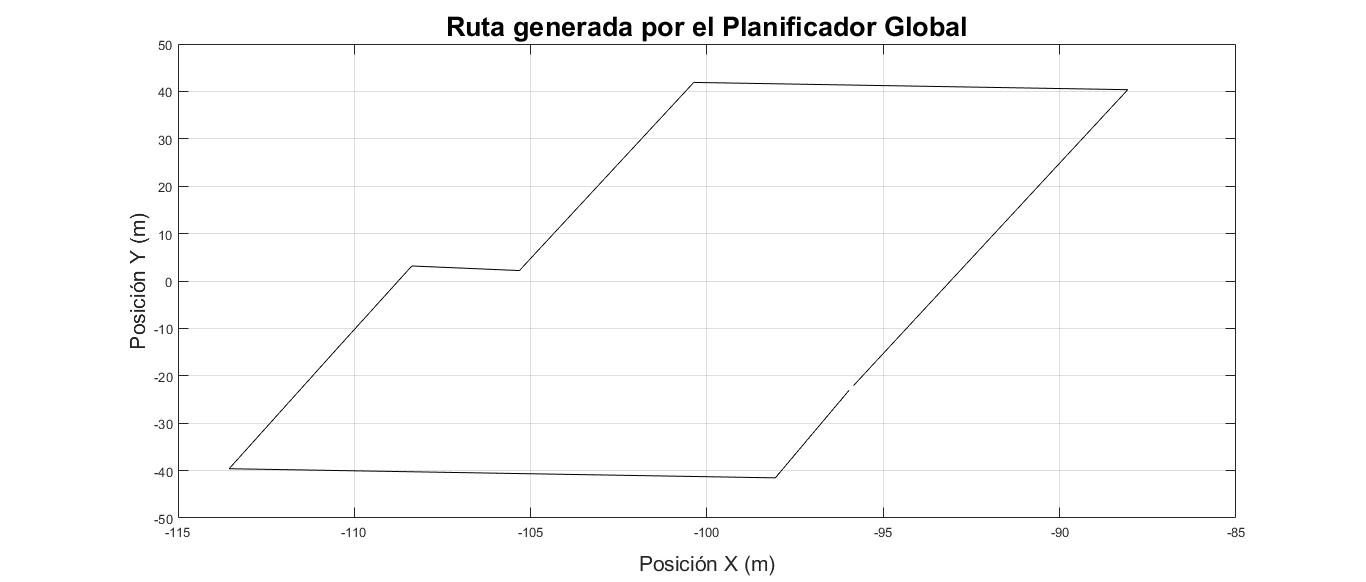
\includegraphics[scale=0.45]{Imagenes/gp}
		\caption{Ejemplo de una ruta generada por el Planificador Global.}
		\label{fig:gp}
\end{figure}	      

	\item Planificador local: basado en la información proveniente del planificafor global, este bloque genera una trayectoria suave empleando curvas paramétricas (Figura \ref{fig:pl}), como es demostrado en \cite{rastelli2014dynamic}. El objetivo es suavizar el cambio de la curvatura entre segmentos rectos y curvas. Este bloque considera la posibilidad de cambiar la trayectoria en caso de que ocurra un escenario ineseperado, como, evasión de objetos, incorporación, entre otros. Para generar este suavizado se emplean por ejemplo las curvas de bezier, como es demostrado en \cite{gonzalez2016review}, las cuales son de fácil implementación y de bajo coste computacional.

\begin{figure}[!h]
	\centering
		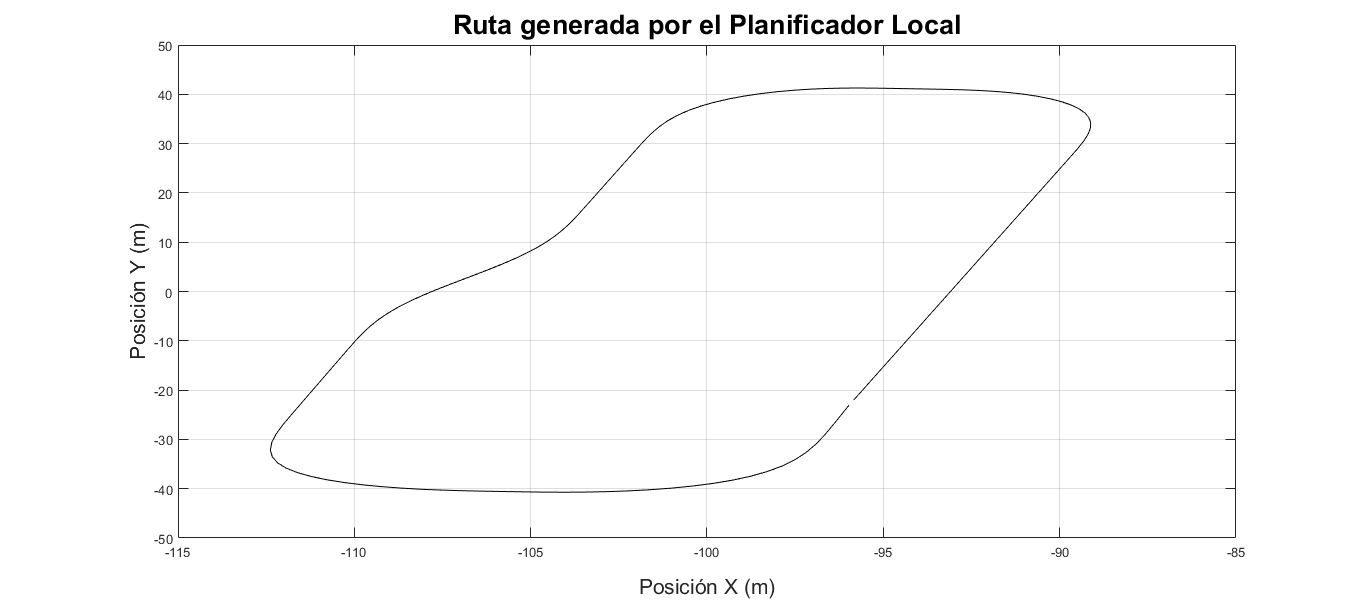
\includegraphics[scale=0.45]{Imagenes/pl}
		\caption{Ejemplo de una ruta generada por el Planificador Local.}
		\label{fig:pl}
\end{figure}	      

	\item \textit{ Buffer} de planificación: es el arreglo empleado para comunicar el bloque de desición con el de control. El mismo pretende optimizar e incrementar el tiempo de respuesta del cálculo de las leyes de control, en caso de detectarse una trayectoria irreal, como un generada con un objeto en frente del vehículo, la mismas es removida antes de enviarse al módulo de control. El \textit{Buffer} está compuesto por: el valor de identificación del punto, tipo de punto, coordinadas X-Y, máxima velocidad del segmento, curvatura y la orientación del segmento.    
	\end{itemize}
	\item Control: es el bloque encargado de realizar el control longitudinal (aceleración y freno) y el control lateral (Volante). Para cumplir este objetivo el módulo recibe el \textit{buffer} de planificación del bloque de desición, con el cual se puede emplear un controlador PID para el control longitudinal, y un controlador basado en la lógica difusa como el mostrado en \cite{perez2013trajectory}, para el control lateral, basado en la utilización del error lateral y error angular. 
	\item Actuadores: es el bloque encargado de normalizar las salidas del módulo de control, con el fin de poder tener señales de acción reales sobre el acelerador, freno y volante. Estas señales son posteriormente enviadas a los respectivos módulos de el vehículo real (actuadores) y virtual (modelo multicuerpo).
\end{itemize} 

\par En la figura \ref{fig:dyna} se puede apreciar la implementación de esta arquitectura en la herramienta Simulink, donde se observan los bloques bien divididos, con sus respectivas conexiones. De este diagrama se resalta el bloque de DynacarJam, el cual es el puente entre el diagrama y el visor 3D, ducho bloque recibe el valor de los actuadores y del volante, entregando un vector con todos los valores necesarios para el movimiento del vehículo en el simulador, siendo el equivalente, el bloque de Twizy V1.0, el cual cumple la función de puente entre Simulink y el vehículo.  	
   
\begin{figure}[!h]
	\centering
		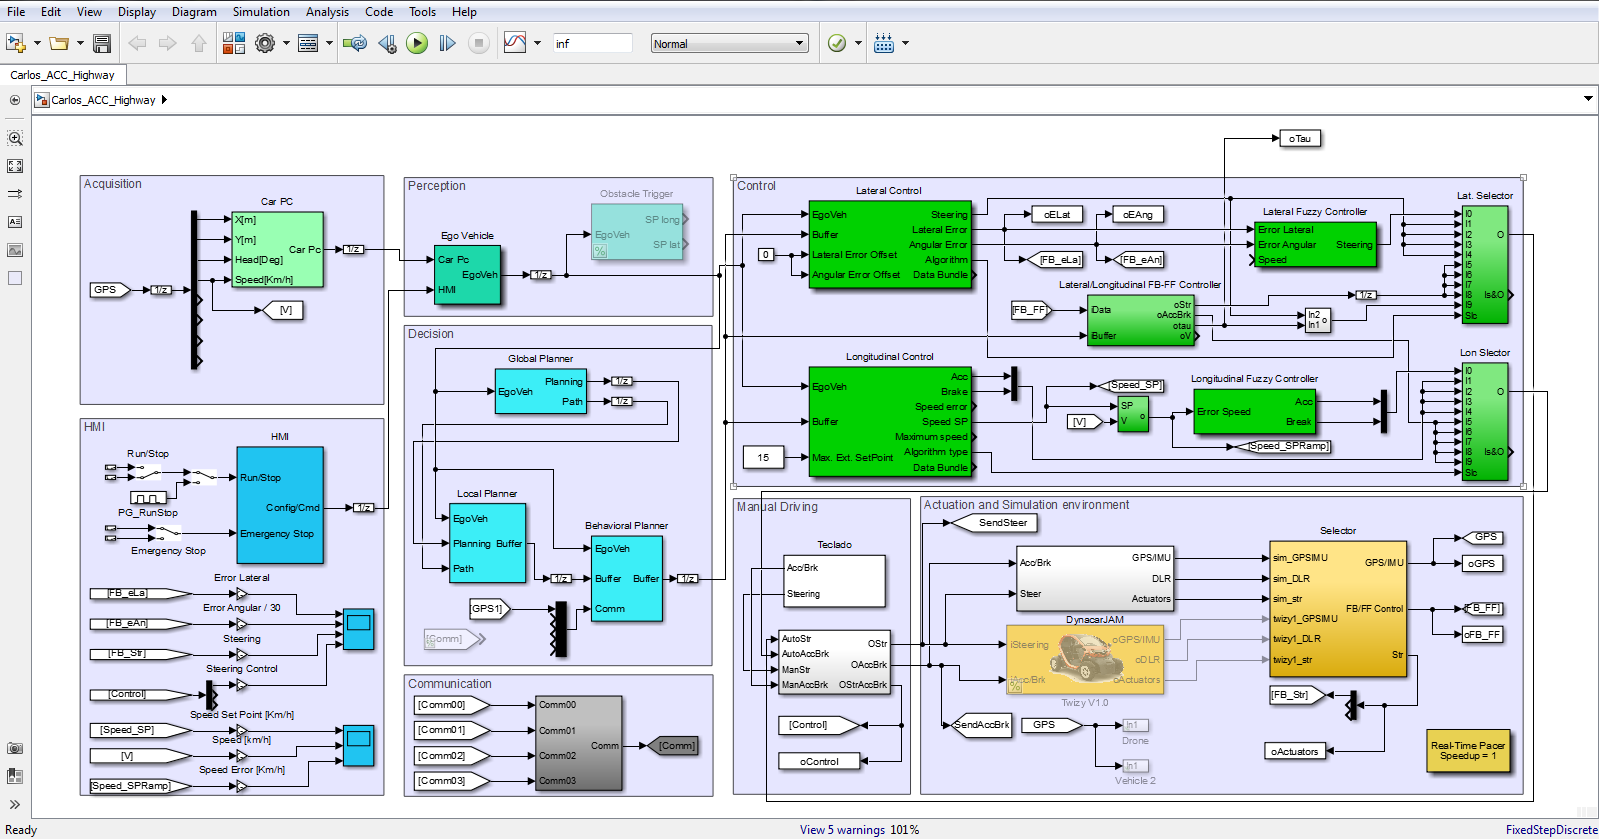
\includegraphics[scale=0.35]{Imagenes/dyna}
		\caption{Arquitectura de control implementada en Simulink}
		\label{fig:dyna}
\end{figure}	
\section{Resumen}
En el capítulo 4 se presentaron las plataformas experimentales empleadas en el transcurso del trabajo. Dentro de estas plataformas se encuentra MATLAB, del cual se resaltaron sus características más importantes, así como los beneficios de poder programar en otros lenguajes. Posteriormente se habló sobre la herramienta Simulink, que debido a su cualidad asíncrona se adapta perfectamente para implementar la arquitectura de control, tanto para el simulador Dynacar, como para los vehículos Twizy. Además, se presentó el simulador Dyancar como una forma de validar los algoritmos propuestos y los sistemas diseñados para vehículos autónomos. Cabe destacar que el mismo provee un entorno 3D, de gran utilidad para monitorear en tiempo real la respuesta de los vehículos en distintas situaciones, así como sus características.\\
\par Finalmente se presentó de forma muy breve la arquitectura de control establecida para la validación de los modelos, en el simulador Dynacar, describiendo cada bloque, así como las conexiones entre cada uno. Además se mostró la implementación de esta arquitectura en Simulink, resaltando la diferencia entre el diagrama empleado en Dynacar y el utilizado en los Twizy.     

